\section{Traceability}
\label{sec:Traceability}

\begin{figure}[!h]
\centering
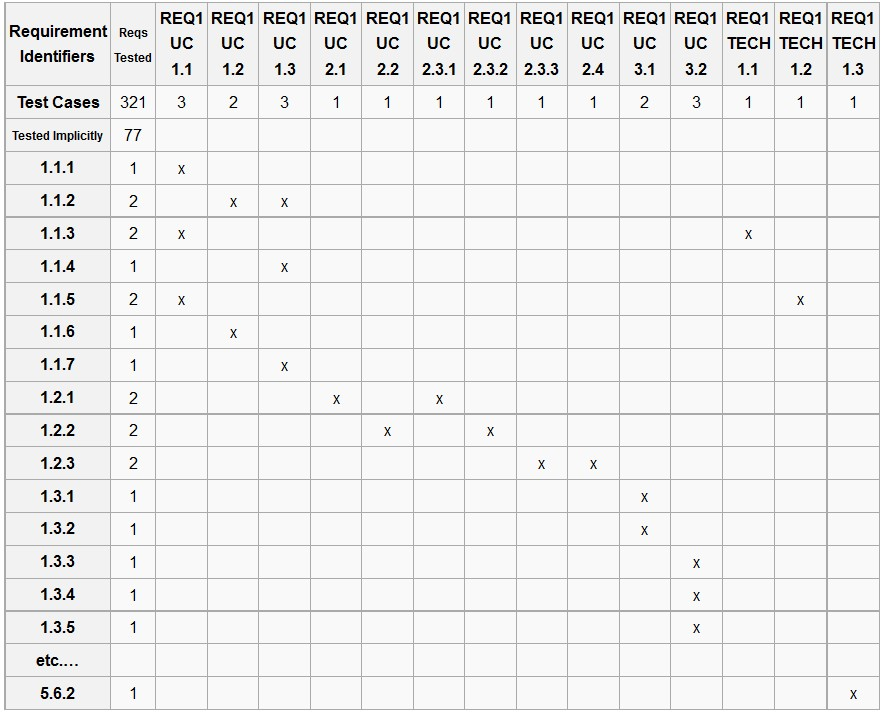
\includegraphics[width=1\linewidth]{TraceabilityMatrix}
\caption{\ttfamily{Traceability Matrix sample}}
\label{fig:TraceabilityMatrix}
\end{figure}

\index{Traceability}Traceability is the ability to identify related items in documentation and software, such as requirements with associated tests.

A traceability matrix is a document, usually in the form of a table, that correlates any two baselined documents that require a many-to-many relationship to determine the completeness of the relationship.

It is often used with high-level requirements (these often consist of marketing requirements) and detailed requirements of the product to the matching parts of high-level design, detailed design, \index{Test Plan}test plan, and \index{Test Case}test cases.

A requirements traceability matrix may be used to check to see if the current project requirements are being met, and to help in the creation of a request for proposal, software requirements specification, various deliverable documents, and project plan tasks.

Common usage is to take the identifier for each of the items of one document and place them in the left column. The identifiers for the other document are placed across the top row. When an item in the left column is related to an item across the top, a mark is placed in the intersecting cell. The number of relationships are added up for each row and each column. This value indicates the mapping of the two items. Zero values indicate that no relationship exists. It must be determined if a relationship must be made. Large values imply that the relationship is too complex and should be simplified.

To ease the creation of traceability matrices, it is advisable to add the relationships to the source documents for both backward traceability and forward traceability. That way, when an item is changed in one baselined document, it's easy to see what needs to be changed in the other.